\documentclass[sigconf]{acmart}
\usepackage{booktabs} % For formal tables
\usepackage{multicol}
\settopmatter{printacmref=false} % Removes citation information below abstract
\renewcommand\footnotetextcopyrightpermission[1]{} % removes footnote with conference information in first column
\pagestyle{plain} % removes running headers
\usepackage[utf8]{inputenc}
\usepackage[english]{babel}
\usepackage{color}
\usepackage{hyperref}
\begin{document}

\title{An autonomous wearable system for posture monitoring and correction during plank exercise using haptic feedback}
\subtitle{Research in Emerging Technologies 2017-2018 }


\author{Ben Monaghan}
\affiliation{%
\institution{Amsterdam University of Applied Sciences}
\department{Software Engineering}
\streetaddress{Wibautstraat 2-4 }
\city{Amsterdam}
\postcode{1091GM}
\country{The Netherlands}}
\email{ben.monaghan2@hva.nl}


\author{Geoffrey Van Driessel}
\affiliation{%
\institution{Amsterdam University of Applied Sciences}
\department{Software Engineering}
\streetaddress{Wibautstraat 2-4 }
\city{Amsterdam}
\postcode{1091GM}
\country{The Netherlands}}
\email{geoffrey.van.griessel@hva.nl}

\author{Peshmerge Morad}
\affiliation{%
\institution{Amsterdam University of Applied Sciences}
\department{Software Engineering}
\streetaddress{Wibautstraat 2-4 }
\city{Amsterdam}
\postcode{1091GM}
\country{The Netherlands}}
\email{peshmerge.morad@hva.nl}

\author{Tom Klootwijk}
\affiliation{%
\institution{Amsterdam University of Applied Sciences}
\department{Game Development}
\streetaddress{Wibautstraat 2-4 }
\city{Amsterdam}
\postcode{1091GM}
\country{The Netherlands}}
\email{tom.klootwijk@hva.nl}

\begin{abstract}
The basis of this project was to find out what type of haptic feedback can help correcting users' posture. Because in modern times where people often sit most of the day, poor posture becomes more and more of a problem. For this purpose, we created a wearable which can autonomously detect the users' posture during a plank exercise. The project aimed to identify which haptic feedback pattern could be the most effective in giving feedback and leading to correct the users\textquotesingle  posture. We have developed an autonomous wearable using an Arduino\footnote{Arduino is micro-controller which can be easily connected to personal computers to be programmed.}, flex sensors\footnote{Flex sensor is a sensor that measures the amount of deflection or bending through the change in Electrical resistance.} , haptic feedback\footnote{Haptic motor is a vibration motor which is widely used in mobile phone and game machines.} motors  and variety fabric belts which are connected to be wearable. We have tested out three different patterns on a total of 13 different users. We have found out that the data varies greatly and not everybody is familiar with the plank exercise which. Because not all users are familiar with this exercise, the test sessions were not all exactly 60 seconds as we have planned. In addition, we have found out the most effective haptic feedback pattern was the guidance pattern, referred to as the second pattern (Pattern 2). Using the second pattern has resulted in a higher time percentage for maintaining the correct posture. Which is the most crucial part while performing a plank exercise. While the users also had to be corrected less than the other patterns.
\end{abstract}


\maketitle
\section{introduction}
 In modern times where people often sit most of the day, poor posture becomes more and more of a problem \cite{subasi2015evaluation}. This can manifest itself in a variety of issues such as neck pain, shoulder pain and lower back pain \cite{hush2006risk, sadeghian2012persistent, o2011association}. One potential prescription for poor posture and its related issues is resistance training \cite{falla2007effect, steffens2016prevention, ruivo2017effects}. Unfortunately, there are numerous barriers to adopting a regular exercise regimen, such as cost, time, distance to suitable gym, lack of confidence \cite{greenwood2015motivators, mailey2016overcoming, sechrist1987development}.  \\


One potential solution to the aforementioned barriers is exercising at home; it removes the time and travel issues associated with going to a gym, and the cost of a gym membership. However, for an at home solution to be effective, the user needs to ensure correct form \cite{winett2001potential}. Something not possible without the presence of an instructor. Improving posture takes effort, either by the user (as in learning how to have correct posture) or by a different person, for instance a personal trainer or a physiotherapist. This can be automated with modern day technologies, like wearables. Possibly cutting costs and increasing accessibility. 

This research aims to see if wearable technology can be used to alleviate barriers to exercise by offering an effective alternative to conventional guided exercise (Such as with a personal trainer). We set out to build a prototype for a wearable shirt that gives haptic feedback to correct posture. With this we can test what type of haptic feedback patterns work best for correcting posture during exercise. Possibly leading us to a device that aids in correcting posture.

Therefore, the main research question of this paper is: What type of haptic feedback patterns is best used in a wearable for correcting posture during a plank exercise? In addition, we have formulated sub questions that will help us answer the research question. These are:
\begin{enumerate}
\item What is correct posture? 
	\begin{enumerate}
		 \item What is correct posture during a plank exercise?
 	\end{enumerate}
\item How can posture be monitored during a plank exercise using sensors?
	\begin{enumerate}
		\item	How to integrate the sensors into a wearable?
	\end{enumerate}
\item How can haptic feedback correct posture during a plank exercise?
	\begin{enumerate}
		\item What is the best moment to give feedback?
 		\item What is the best haptic pattern to give feedback during a plank exercise?
 		\item What are effective spots of the body to give feedback during a plank exercise?
 	\end{enumerate}
\item What are the results of the different haptic feedback patterns on posture?
\end{enumerate}

\section{Related work}
There have been a number of studies in how to monitor posture, however these appear to be mostly focused on classifying spine position in a clinical setting, with limited carryover to being used for exercise and home usage 
\cite{wong2008detecting,voinea2016measurement, wong2008smart} 
Specifically, they focus on doctor/patient scenarios for rehabilitation/physiotherapy and not for general, unsupervised usage. As a result these are often cumbersome and require expert knowledge to apply.  There has been some work in creating a user friendly system \cite{sardini2015wireless} using an inductive sensor sown directly into a T-Shirt, resulting in a less intrusive way of monitoring spine position.  
Haptic feedback has been studied in a variety of safety critical applications, such as in cars and planes 
\cite{goodrich2004learning, hannaford2004proceedings}. However the mechanism for feedback is only as a warning system, and not a means of guiding movement. There appears to be limited research specifically related to haptic feedback and exercise. As far as we could tell there are two relevant studies, which includes ensuring exercise intensity is maintained using a variety of feedback protocols \cite{ferber2007using} and directing shoulder flexion and extension \cite{alizadeh2014haptics}.
These suggest that feedback should be limited to correction (that is, not constantly on) which potentially rules out positive feedback (I.E there is constant vibration if the user is in the correct position) as it causes annoyance. 
The Literature review shows that there has been little research into combining haptic feedback and a monitoring system to correct posture in real-time. From what we can see, there has been one study that achieves this aim in a single device \cite{zheng2010vibrotactile}.  However, this is limited to only static posture (sitting) and is in the form of an external (a chair) device. 
We intend to build upon the concepts developed in \cite{ferber2007using} by incorporating different feedback patterns with a wearable, which includes the functionality to detect whether posture is incorrect or correct. 


\section{Method}
This research is an experimental research. We have made a prototype which can help us identifying which haptic feedback pattern is the most effective in correcting users' posture. We have prepared test sessions where the participants were asked to do a plank exercise wearing the prototype. The aim of these sessions was to gather quantitative data which can be used later to reach our goal.  We had 13 participants who have done the plank exercise. We have processed the gathered data and analyzed it. Then we draw an objective conclusion based on the statistics we obtained. 


\section{What is correct posture? }
Correct posture can be defined as a position which ensures the natural curvature of the spine, specifically an  \textquotesingle S \textquotesingle shape starting from the base of the neck (Cervical region), a slight convex bend in the upper back (Thoracic region) and a concave bend in the lower back (Lumbar region).  The ideal position is neutral. That is, no extension or flexion in the upper and lower back, and no lateral movement \cite{activaided}.

\begin{figure}[h]
\centering
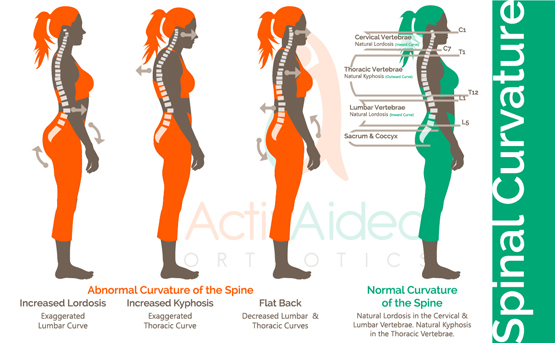
\includegraphics[width=0.45\textwidth, scale=1]{CorrectPosture.png}
\caption{Correct posture \cite{activaided} }
\end{figure}


Within the context of sports and exercise, this correct posture remains the same as in just general day to day activities (I.E the S shape of the spine is maintained). This is considered the optimal position for force transferal from the feet to the upper limbs, paramount in almost any sport (such as a rugby player in a scrum or a shotput thrower in the Olympics), as well as means to reduce injury rates \cite{videman1997lifetime}.  Any flexion, extension or lateral movement can cause pressure on the intervertebral discs, causing them to protrude (I.E a trapped disc, or herniated disc), putting pressure on the nerve roots running throughout the spine \cite{videman1997lifetime}. 

A plank exercise consists of lying on the floor in the prone position, then rising onto the elbows, arms extended out in front (so the elbow is 90 degrees to the floor), legs fully extended behind and on the tips toes. It is an isometric exercise specifically for training the core{-}a common way of describing the muscles which provide trunk stability such the lower back muscles and the abdominals.  The isometric nature of the exercise makes it a popular choice for training the lower back and abdominal as it closely emulates their primary function{-}maintaining a neutral spine. With that in mind, the optimal posture for a plank position is also the same for when stood up, that is, to maintain the natural S shape of the spine, while keeping a neutral pelvis position \cite{cortell2017influence}.

\section{How can posture be monitored during a plank exercise using sensors?}

There have been a number of studies in how to monitor posture, however these appear to be mostly focused on classifying spine position in a clinical setting, with limited carryover to being used for exercise and home usage  \cite{wong2008detecting, voinea2016measurement, wong2008smart} . Specifically, they focus on doctor/patient scenarios for rehabilitation/physiotherapy and not for general, unsupervised usage. As a result, these are often cumbersome and require expert knowledge to apply. There has been some work in creating a user{-}friendly system \cite{sardini2015wireless} using an inductive sensor sown directly into a T{-}Shirt, resulting in a less intrusive way of monitoring spine position.   

\subsection{The prototype}

We intend to use a method similar to the method shown in \cite{sardini2015wireless}, however instead of using inductive sensors sown for the full length of the spine, we have identified three locations where movement can occur which moves the wearer outside of correct posture – the upper, middle and lower regions of the back. At each region we had to attach a flex sensor (A variable resistor which changes resistance as it bends). See figure 1.  For our purposes we do not need to map the curvature of the spine as is required in medical settings. We simply need to know if the back is bending. If so, we notify the wearer. Flex sensors can provide enough sensitivity that we can create a range that allows for different wearers (not all backs have the same curvature) to calibrate it to themselves. It was impractical to use gyroscopes or accelerometers, this because they are affected by drift over time. \cite{papi2017wearable}  Next to that we avoided the use of strain gauges, as they would have to be placed meticulously on the body for it to read correct values. \cite{papi2017wearable} This would have been to impractical to put on and use. The only robust option left at our disposal was the flex sensor.

To house the flex sensors we will use a belt with attached straps, for practical and hygienic reasons. The belt can easily be taken off and be attached to a different user. There will have to be two haptic feedback motors per flex sensor, to make sure that the device gives off enough feedback. Even through multiple layers of clothing. The choice to use haptic feedback was made over visual or auditory feedback because of the intuitive response of the body and position specific feedback. The user will feel the point that will have to be corrected and adjust accordingly.
\begin{figure}[h]
\centering
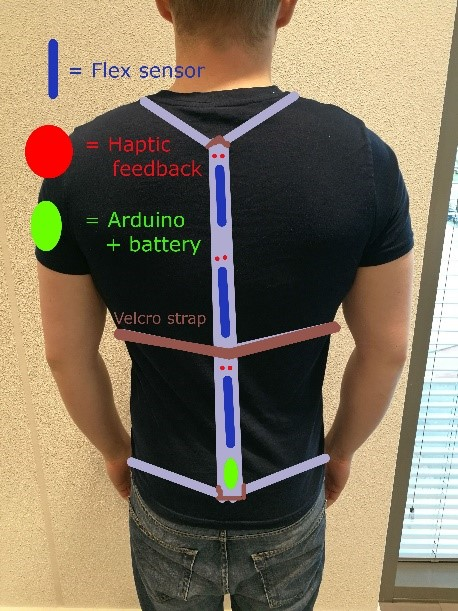
\includegraphics[scale=1]{Ben_Prototype.jpg}
\caption{The design for the belt.}
\end{figure}


The final belt for the prototype largely follows the original design. The only two differences are that the strap in the middle is moved slightly downwards so it pulls the belt into the curve of the lower back. Besides that, the haptic motors are moved next to the flex sensors. This will allow the feedback to be more in line to the exact point where the curvature is measured.


\begin{figure}[h]
\centering
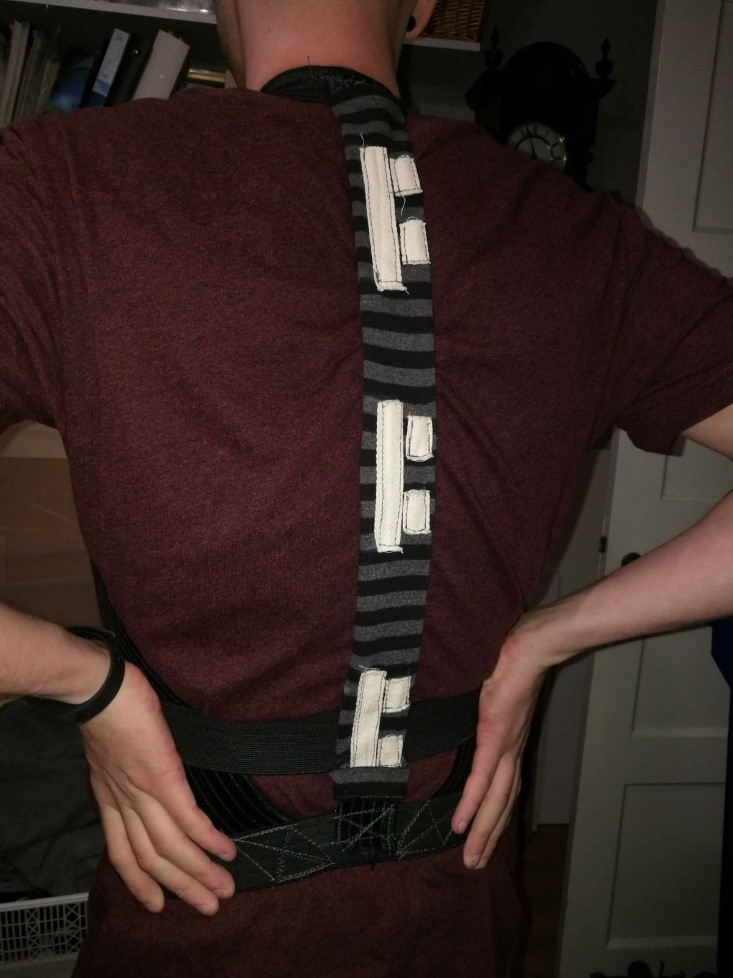
\includegraphics[width=0.25\textwidth, scale=0.5]{Tom_Prototype.jpg}
\caption{The actual belt for the prototype}
\end{figure}

\begin{figure}[h]
\centering
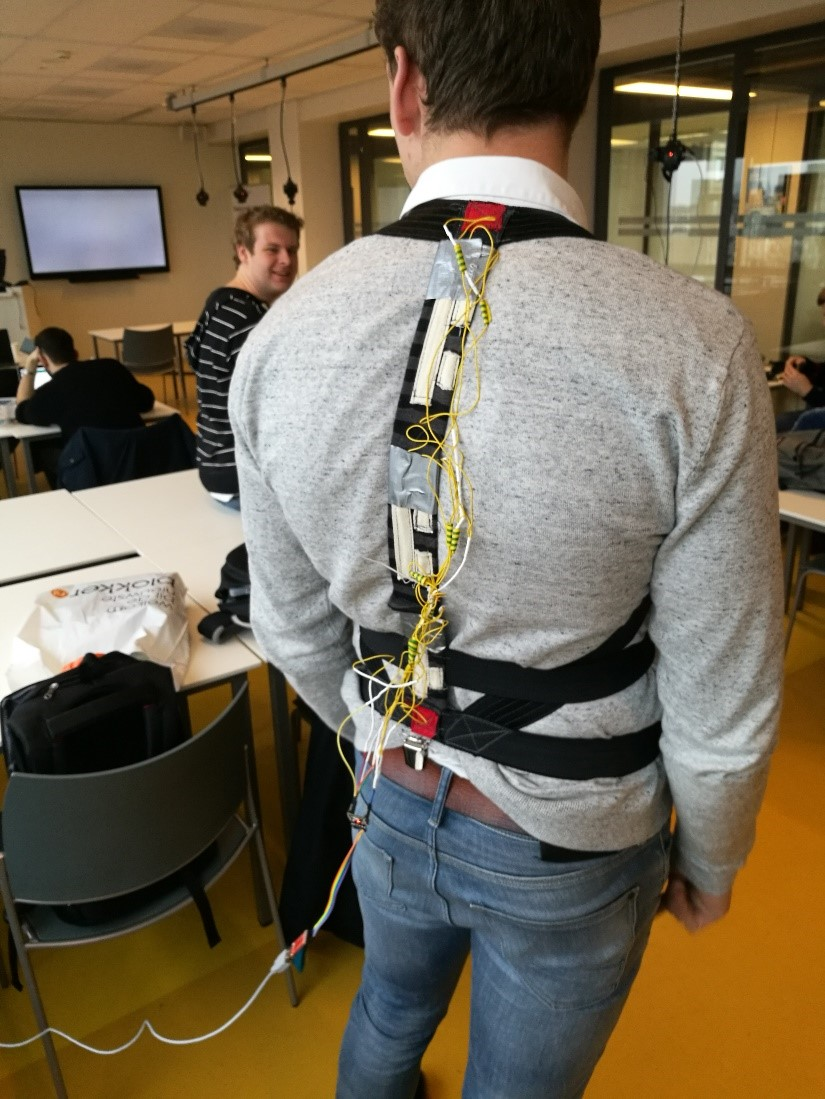
\includegraphics[scale=0.5]{Mattijs_Prototype.jpg}
\caption{: The prototype during a test session}
\end{figure}

Besides the flex sensors and haptic feedback motors, an Arduino pro mini was used. There are various micro controllers out there, but the Arduino pro mini was easily obtainable for us. As well as it has the perfect form factor for a prototype like this. The differences between microcontrollers is neglectable for our purpose.
On the software side (Github repository can be found at: \url{https://github.com/geoffreyvd/posture-helper-wearable} ), the user can start recording the current state/position of the spine by pressing a button. This will save the values of the flex sensor. These values are used to determine if a part of the spine is too much out of place. Flex sensors have a specific value for a corresponding specific angle. The more a flex sensor bends the more the resistance is increased. As such the voltage read on the pin of the Arduino differs, which in turn corresponds to a specific angle.

\begin{figure}[bh]
\centering
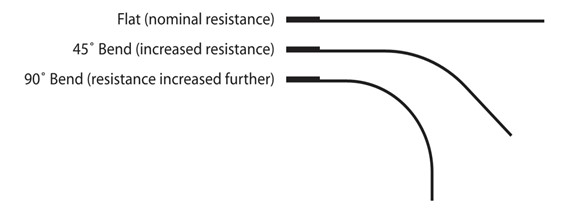
\includegraphics[width=0.5\textwidth, scale=1]{FlexSensor_work.jpg}
\caption{How a flex sensor works.}
\end{figure}


Every loop the Arduino checks if the current angle/value reported by the flex sensor is higher than a certain threshold, if it is then it will trigger feedback. What type of feedback given is dependent on the specific pattern that's active. A separate class manages the active feedback pattern and controls the associated feedback motors. The feedback stops when the specific flex sensor is near the original calibrated angle again (within the threshold). The feedback motors are controlled with PWM (Pulse Width Modulation) for the patterns that require more precise control rather than just being turn on or off.
The device is autonomous except for the user having to pick a specific position (preferably correct posture) and record this to use as calibration. This is unavoidable. Besides that, the prototype functions as expected.
Furthermore, for the data gathering part a separate Java program was built that can log the data at specific time intervals in to a CSV file. This was the data that could be easily analyzed at the end of the testing. At a specific time interval the Arduino writes the data over serial communication to the computer. The Java program records this data and stores it in the CSV file.
And to conclude we made a tool in Python that analyses the data gathered by the Java program and returns the metrics that we are looking for.

\section{How can haptic feedback correct posture during a plank exercise?}
Haptic feedback has been used in a variety of industries, from gaming (such as vibrating control pads), to healthcare \cite{bethea2004application}, to mobile \cite{cuartielles2012mobile}, to the military and aerospace industries.  All with different aims. Gaming focuses on providing feedback to give a sense of immersion –a controller vibrates when an explosion appears on screen for instance. Healthcare aims to emulate the feedback during remote operations (such as the resistance of tissue if cutting with a scalpel). The military \cite{immonen2008haptics} and aerospace have both attempted to both use it as a means of notification and a way of providing guidance. Haptic feedback can offer an added benefit over typical methods (Audio, visual) as it has a reduced cognitive load, therefore in high intensity environments (such as a fighter pilot) it can serve as a suitable method for giving feedback, without increasing the cognitive load required to process it.\\

The locations have been decided in line with how we are intending to monitor the wearer\textquotesingle s posture, so one sensor and haptic at the top, middle and lower back regions.
We have a mix of alert (such as in gaming controllers), guidance (such as in the military) and a simple linear increasing pattern. To this end we used the following types of haptic feedback:

\subsection{Linear increasing}
This haptic pattern simply increases the intensity of the feedback when the input (flex sensor angle) increases. So the more a posture deviates from correct posture, the stronger the vibration. This happens in parallel, so each haptic will represent its angle at the same time.

\subsection{Guidance}
This will consist of alternating the intensity of the feedback to give the feeling of guidance (very similair to pulsing). For example, starting at a low intensity and increasing to high might give the impression of being \textquotesingle pushed \textquotesingle down, conversely starting high and moving to low might give the impression of being \textquotesingle pulled \textquotesingle up. As with the alert patterns, these can be both tested in sequence and in parallel. This provides an opportunity to see if firstly, can haptic feedback guide a wearer into the correct position and secondly, can a wearer receive feedback at two various locations without causing confusion.\\

\subsection{Alert}
This will consist of simple feedback – a vibrating motor – when the wearer is not in the correct position, so vibration is either on or off. There are two possible protocols, alert in sequence and alert in parallel. Alert in sequence will alert the wearer at one and only one of the three points (upper, middle, lower back) until they have moved into the correct position, then, if needed, move to the next position and provide feedback at that point, working in sequence until all three are in position. Alert in parallel will provide simultaneous feedback at all three points. For instance, using the in sequence method, if the wearer\textquotesingle s upper back is in flexion and their lower back then moves into extension, the feedback will first start at the upper back region, then when that is correct, begin at the lower region. Conversely, the parallel feedback will alert the wearer at both regions simultaneously. 



We are using three patterns for our tests: the linear increasing, parallel pushing guidance and parallel alert patterns, these will be referred to as pattern1, pattern2 and pattern3, respectively. For each pattern we took into account that a flex sensor might return a range of a minimum of {-}10 degree to a maximum of 90 degree, where 0 degree is the calibrated flex value(a flex sensor value for that specific user that indicates good posture). 
Example: for pattern1 the base is 0 and flex sensor value deviation from that will result in an linear increasing vibration for the according haptic motor. For the other two patterns we use a threshold of 35 which comes down to the first \textasciitilde 7 degrees.


\section{What are the results of the different haptic feedback patterns on posture?}
For the purpose of knowing which pattern is the most effective in correcting users\textquotesingle posture, we have setup test sessions. 
We have used Processing \footnote{Processing is an open{-}source computer programming language and integrated development environment (IDE) built for the electronic arts}  to capture the data, read the values of flex sensors from the serial port, and store them into files which can be read later by any programming language for data analysis purposes. In each file the used pattern and user calibration is also stored.

\subsection{Testing}
After proposing multiple patterns, we tested them on a group of subjects. The group consisted of 13 people, aged 19 – 25 and all with various levels of fitness. The test consisted of performing a plank exercise three times while wearing the posture correction wearable which was configured with one specific pattern per plank exercise attempt. It is important to note that the results discussed next are obtained from testing sessions which lasted 60 seconds on average.
A related point to consider here is that not every person could perform the plank exercise well. The plank exercise was challenging for large group of the test participants. 

The reason we picked a group of 13 people with such varied backgrounds is that people with posture problems will all be very different from each other in what kind of problems they have. Compared to say for instance amputees that are missing their complete left leg. Which would be more specific. Even though the group was varied, every single person tried out the three patterns, as such the data is not skewed in that sense.

We ended up selecting a handful of people from our class with varied backgrounds, and a handful of strangers. To keep the results somewhat mixed. The reason we picked 13 people is that we decided we needed at least 10 sets of data to be able to draw averages from the statistics, several more people were willing to participate luckily.
We are interested in the following information retrieved from analyzing the data of the different patterns:

\begin{enumerate}
\item How many times did the user have to be corrected, per flex sensor?
\item On average, how long did it take before the user corrected him/herself?
\item How much of the total time did they maintain correct posture? 
\end{enumerate}

The answer to the first question will be a list of three values. Each value represents correction frequency for a flex sensor. 
The answer to the second question will be in milliseconds. It is one value and it an average of the required time to before the user corrected him/herself. It is a duration that starts when the user enters the state \textquotesingle incorrect posture\textquotesingle and ends when the user corrects the posture. 
In contrast to the second question, the answer to the third question is percentage of time the user was in the state \textquotesingle correct posture\textquotesingle. 

We will start off by listing the results per pattern basis. After which we will compare the gathered information to each other and rank the different patterns. The next step after gathering the data is analyzing the data and convert them into information which can help us determine which used pattern has worked most effectively in correcting the user\textquotesingle s posture during doing the plank exercise. For that purpose, we have developed our own data analysis script that helped us to give answers to the above{-}mentioned questions. 

\subsubsection{Testing outcomes} 
We present a table with results and a bar chart for each question to make the results clear and readable. The three values in the first column of the table are respectively the values from flex sensors 1, 2 and 3.\\

For analyzing the data, generating information and generating charts we have used Python \footnote{Python is an interpreted high{-}level programming language for general{-}purpose programming}. We made our own data analysis tool for that purpose. 
The code is hosted on Github \\ 
\url{https://github.com/peshmerge/infonl_graphs} \& \\
\url{https://github.com/peshmerge/infonl_stats} 


%Pattern1
\paragraph {\textbf{Pattern1}}
Table of average physical results of all users for this pattern.
\begin{table}[h]
\caption{Pattern 1 and detailed answers in number to the formulated questions}
\label{my-label}
\begin{tabular}{|l|l|l|}
\hline
\multicolumn{1}{|c|}{\textbf{First question}} & \multicolumn{1}{c|}{\textbf{Second question}} & \multicolumn{1}{c|}{\textbf{Third question}} \\ \hline
 [43.0,28.0,32.0]& 10427.648ms & 22\%  \\ \hline
\end{tabular}
\end{table}



Detailed view per statistic
\begin{figure}[h]
\centering
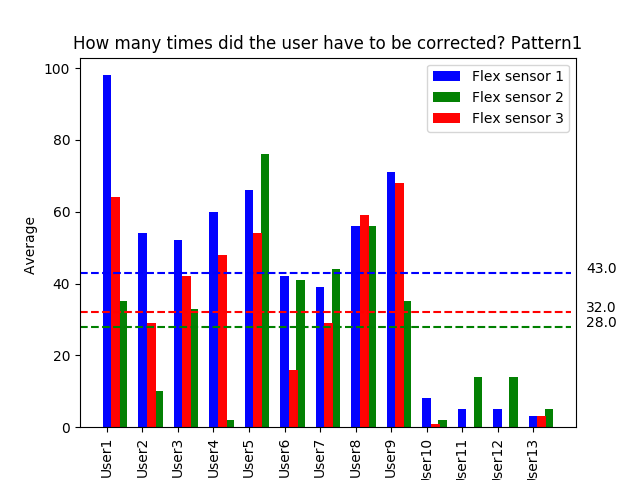
\includegraphics[width=\columnwidth , scale=1]{p1_q1.png}
\caption{How many times did the user have to be corrected?}
\end{figure}

\begin{figure}[h]
\centering
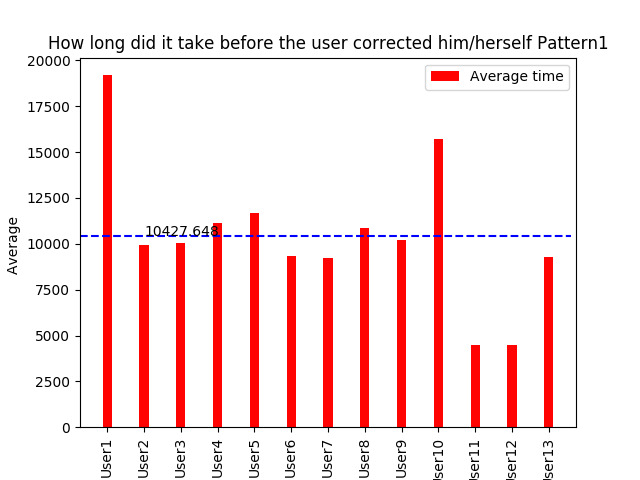
\includegraphics[width=\columnwidth, scale=1]{p1_q2.png}
\caption{On average, how long did it take before the user corrected him/herself?}
\end{figure}

\begin{figure}[h]
\centering
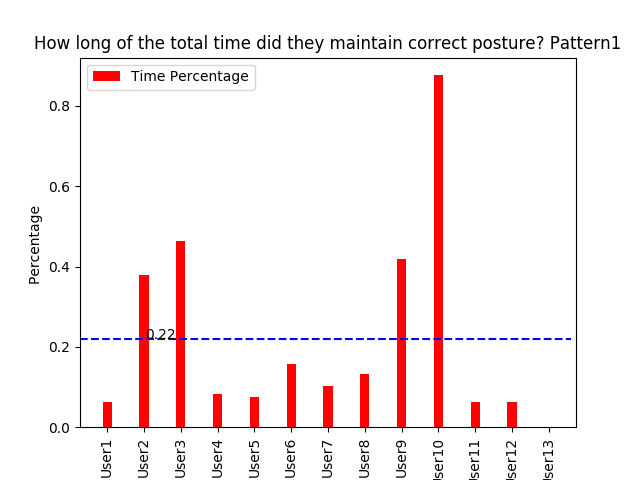
\includegraphics[width=\columnwidth, scale=1]{p1_q3.png}
\caption{On average, how long did it take before the user corrected him/herself?}
\end{figure}
\pagebreak



%Pattern2
\paragraph {\textbf{Pattern2}}
Table of average physical results of all users for this pattern.\\
\begin{table}[htb]
\caption{Pattern 2 and detailed answers in number to the formulated questions}
\label{my-label}
\begin{tabular}{|l|l|l|}
\hline
\multicolumn{1}{|c|}{\textbf{First question}} & \multicolumn{1}{c|}{\textbf{Second question}} & \multicolumn{1}{c|}{\textbf{Third question}} \\ \hline
 [24.0, 26.0, 22.0]& 11931.046 ms & 35\%  \\ \hline
\end{tabular}
\end{table}

Detailed view per statistic
\begin{figure}[hb]
\centering
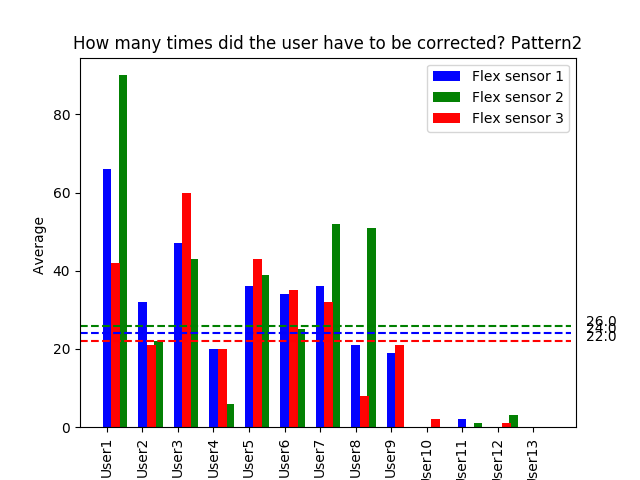
\includegraphics[width=1\columnwidth, scale=1]{p2_q1.png}
\caption{How many times did the user have to be corrected?}
\end{figure}
{\color{white} A blank space } \linebreak

\begin{figure}[ht]
\centering
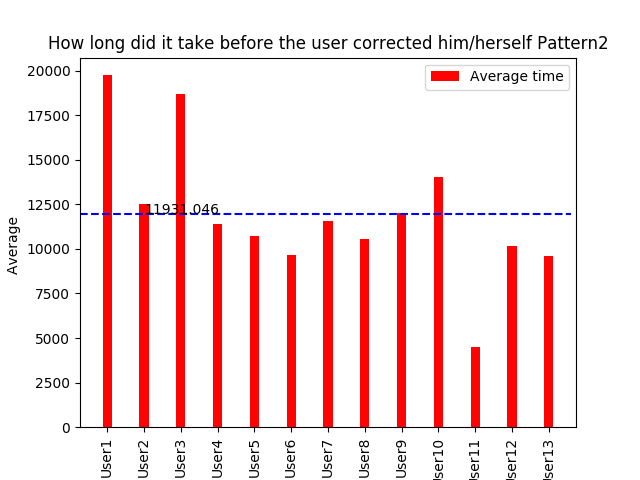
\includegraphics[width=1\columnwidth, scale=1]{p2_q2.png}
\caption{On average, how long did it take before the user corrected him/herself?}
\end{figure}


\begin{figure}[h]
\centering
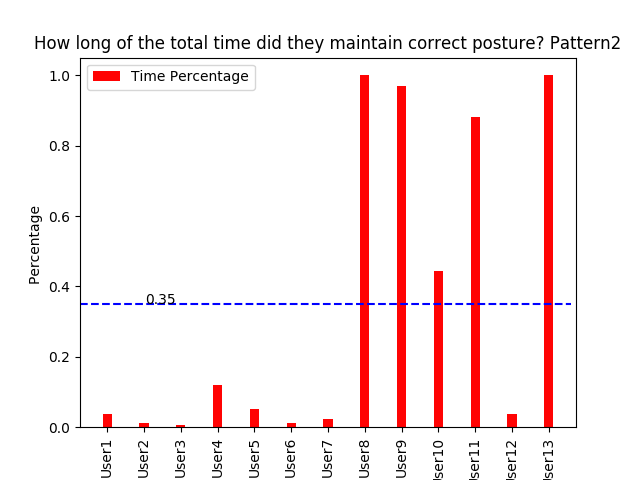
\includegraphics[width=1\columnwidth, scale=1]{p2_q3.png}
\caption{On average, how long did it take before the user corrected him/herself?}
\end{figure}


%Pattern3
\paragraph {\textbf{Pattern3}}
Table of average physical results of all users for this pattern.\\
\begin{table}[htb]
\caption{Pattern 3 and detailed answers in number to the formulated questions}
\label{my-label}
\begin{tabular}{|l|l|l|}
\hline
\multicolumn{1}{|c|}{\textbf{First question}} & \multicolumn{1}{c|}{\textbf{Second question}} & \multicolumn{1}{c|}{\textbf{Third question}} \\ \hline
 			[27.0, 34.0, 22.0]				  & 10851.408 ms 								  &   	12\%  							      \\ \hline
\end{tabular}
\end{table}

Detailed view per statistic
\begin{figure}[ht]
\centering
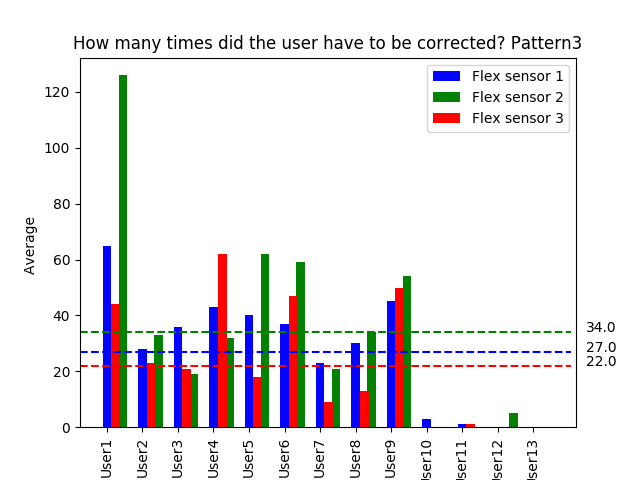
\includegraphics[width=0.8\columnwidth, scale=1]{p3_q1.png}
\caption{How many times did the user have to be corrected?}
\end{figure}

\begin{figure}[h]
\centering
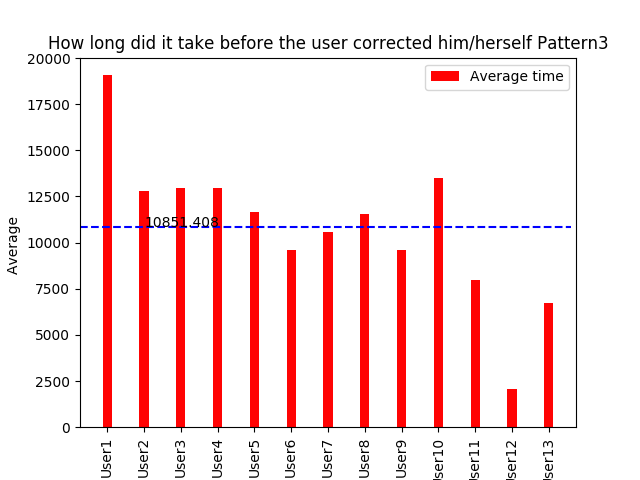
\includegraphics[width=0.8\columnwidth, scale=1]{p3_q2.png}
\caption{On average, how long did it take before the user corrected him/herself?}
\end{figure}


\begin{figure}[h]
\centering
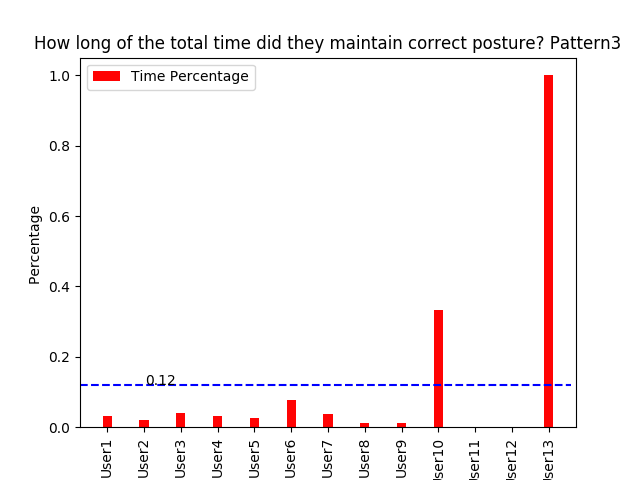
\includegraphics[width=0.8\columnwidth, scale=1]{p3_q3.png}
\caption{On average, how long did it take before the user corrected him/herself?}
\end{figure}
\pagebreak

{\color{white} A blank space } \linebreak
{\color{white} A blank space } \linebreak

%Comparison
As we noticed in the tables and graphs, the data varies greatly. Hence it is important to present the results in a more readable way. We can now compare the data and see which pattern is statistically the best for correcting users’ posture based on the results of the tests sessions.

\begin{table}[h]
\centering
\caption{Used Patterns and the formulated questions.}
\label{my-label}
\begin{tabular}{|l|l|l|l|}
\hline
Pattern & \multicolumn{1}{c|}{\textbf{First question}} & \multicolumn{1}{c|}{\textbf{Second question}} & \multicolumn{1}{c|}{\textbf{Third question}} \\ \hline
First   &  [43.0, 28.0, 32.0] 						  &				10427.648 ms		  			  &		22\%                          \\ \hline
Second  &  [24.0, 26.0, 22.0]              			  &  			11931.046 ms                      &     35\%                           \\ \hline
Third   &  [27.0, 34.0, 22.0]                         &       		10851.408 ms                      &     12\%                            \\ \hline
\end{tabular}
\end{table}

\begin{figure}[h]
\centering
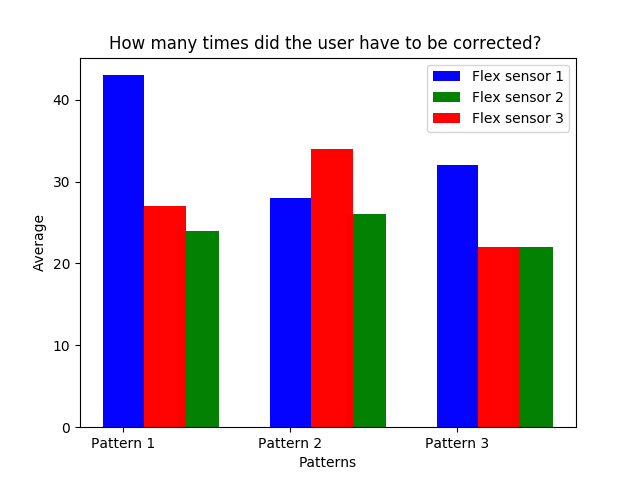
\includegraphics[width=1\columnwidth, scale=1]{p_q1.png}
\caption{On average, how long did it take before the user corrected him/herself?}
\end{figure}

\begin{figure}[hb]
\centering
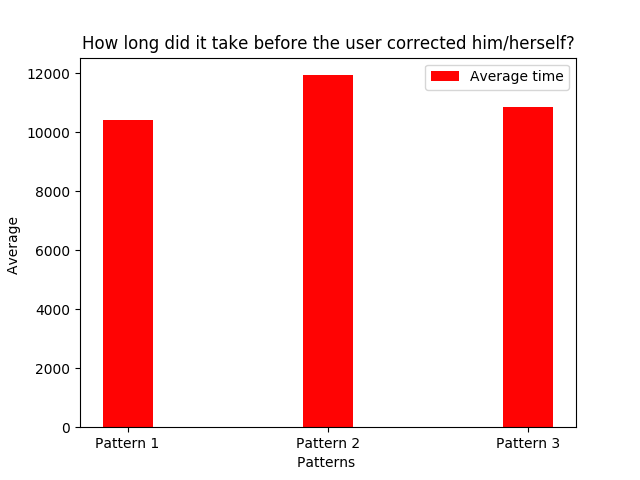
\includegraphics[width=1\columnwidth, scale=1]{p_q2.png}
\caption{How much of the total time did they maintain correct posture?}
\end{figure}

\begin{figure}[h!]
\centering
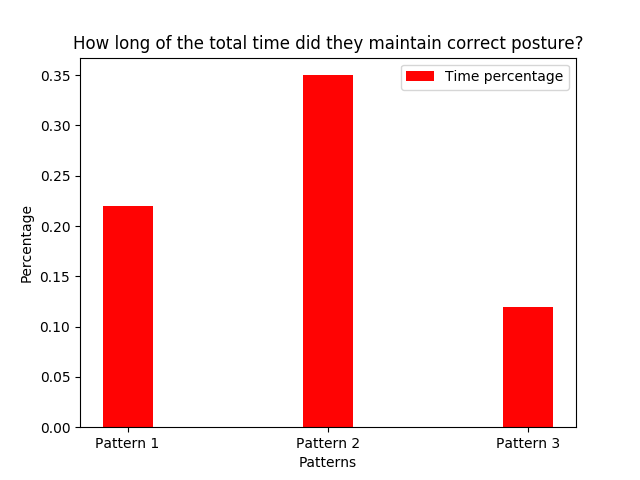
\includegraphics[width=1\columnwidth, scale=1]{p_q3.png}
\caption{How many times did the user have to be corrected, per flex sensor?}
\end{figure} 


Looking solely at the percentage of the time the user maintained correct posture, which is critical for performing a correct plank exercise and putting stress on the correct muscles, pattern two seems to be the best pattern. Even though the average time before the user corrected him/herself was higher than the other patterns they clearly held their posture correctly a higher percentage of the total time. As for the amount of times the user had to be corrected, pattern two was the lowest (lower being better at this statistic) than both patterns. Pattern one had 103 total corrections on average, pattern two had 72, and pattern three had 83. The high number of corrections for pattern 1 might be due to the subtle feedback it gives compared to the other two, which gives the user a clearer idea of where bad posture is.
Based on the statistics, pattern two is clearly the better pattern.


\section{Discussion}
In section seven we defined three questions to help us understand the data we have gathered during testing sessions. The third question is critical in helping us to decide which pattern act as the most effective pattern in correcting the posture. As it is the primary statistic to determine how well the plank exercise was performed. One could try to argue that it is not about keeping the most correct posture, but how well the person responded to feedback and if the user corrected himself accordingly. But this is not the thing that is important with a plank exercise. Keeping form is more important than how many times a person correct himself. Bad posture during exercise could lead to damage to the spine and other injury's. [22] So the more time a user holds his correct posture and the fewer times the user has to be corrected the better. Which clearly shows that pattern two is the better pattern.
The second question is also useful to determine the intensity of the feedback which lead the user to correct their posture in shorter time. One could say that this statistic shows how well the user could perceive the feedback and work to adjust accordingly. This might mean that pattern two does not give the best feedback in terms on intensity or pattern, as it has the worst score out of the three. But it can also mean that the feedback was subtler and with minute changes, which would take the user more time to process than a more intense pattern. But give the user more precise information on how to correct him/herself. A reasonable case could be made about this argument because of the statistics for the other two questions, which clearly show that the users of pattern two both had to be corrected fewer times and that they maintained their overall posture better than the other patterns.
If we look at another patterns point of view, for instance pattern one, it also had a decent total percentage of time where the users maintained correct posture. Nowhere near the percentage of pattern two, but still decent. It did however have the lowest time before the user correct him/herself compared to the other two patterns. Which seems like the pattern has a good feedback pattern/intensity. The problem however is that the total times the user had to be corrected is way higher. Which could be interpreted as the user not getting accurate feedback, but only more intense feedback. Besides that, the total time the users had correct posture is not high enough to even realistically consider this pattern.


\section{Conclusion}

With this research we have aimed to answer the following question: "What type of haptic feedback patterns is best used in a wearable for correcting posture during a plank exercise?".  
To answer this question, we first defined what correct posture is during a plank exercise which turned out that the ideal position is neutral (the shape of an S). That is, no extension or flexion in the upper and lower back, and no lateral movement. Any flexion, extension or lateral movement could cause pressure on the intervertebral discs, causing them to protrude (I.E a trapped disc, or herniated disc), putting pressure on the nerve roots running throughout the spine. 
Then we examined how we can use haptic motors to give useful feedback to the user and defined several feedback patterns to achieve this. We have decided to use the linear increasing, guidance and alert haptic patterns.  
In addition, we have created a prototype which came with a couple of challenges, such as; how to measure posture autonomously and how to be able to calibrate the prototype autonomously such that it can decide properly what the correct posture is. For this purpose we used the Arduino in combination with three flex sensors and three haptic motors, which measures the posture and thereafter gives haptic feedback based on the calibration values.\\  
Subsequently we implemented three haptic patterns and tested those on 13 subjects during a plank exercise. Following the data analysis, we concluded that subjects using the guidance pattern (pattern 2) were the most successful in maintaining correct posture, compared to the linear increasing pattern and alert pattern. We also had to conclude that unfortunately the prototype is not usable for people shorter than 1.65m, and that the prototype really shines with correcting posture while sitting and standing. However, the prototype is a bit less than optimal in a plank position. \\
For future studies we would recommend to use stronger haptic motors if subjects are being tested during exercises. Besides, a future research can examine using longer flex sensor which can more space on the spine. A longer flex sensor means detecting a wider range of changes which can lead to better monitoring. Additionally, future studies could compare the haptic patterns to a "no pattern" baseline, to verify if haptic patterns actually have any positive effect at all during a plank exercise, instead of just comparing different patterns.

\section{Acknowledgment}
This research was supported by Amsterdam University of Applied Sciences and Info.nl. 
We thank Wouter Meys and Annette Brons from Amsterdam University of Applied Sciences for assistance during the research.
We thank Ashlee Valdis from Info.nl for helping us to get all needed hardware to build the prototype. 
We thank all awesome people from the Makers Lab who helped us in wiring and soldering the prototype. 
Finally, We would also like to show our gratitude to all participants who helped us to test our final prototype. 



\bibliographystyle{ACM-Reference-Format}
\bibliography{ReferencesHaptify}

\end{document}